\chapter{Практические задания}

\section{1. Используя только функции CAR и CDR,
написать выражения, возвращающие:}

a) второй
\begin{lstlisting}[language=Lisp]
;; CDR от '(a b c d e f) вернет хвост (b c d e f)
;; СAR от '(b c d e f) вернет голову b (Т.е. второй элемент)
(CAR (CDR '(a b c d e f)))
\end{lstlisting}

b) третий
\begin{lstlisting}[language=Lisp]
;; CDR от '(a b c d e f) вернет хвост  (b c d e f)
;; CDR от '(b c d e f) вернет хвост  (c d e f)
;; СAR от '(c d e f) вернет голову с (Т.е. третий элемент)
(CAR (CDR (CDR '(a b c d e f))))
\end{lstlisting}

c) четвертый элементы заданного списка.
\begin{lstlisting}[language=Lisp]
;; CDR от '(a b c d e f) вернет хвост  (b c d e f)
;; CDR от '(b c d e f) вернет хвост (c d e f)
;; CDR от '(b c d e f) вернет хвост (d e f)
;; СAR от '(d e f) вернет голову d (Т.е. четвертый элемент)
(CAR (CDR (CDR (CDR '(a b c d e f)))))
\end{lstlisting}

\section{Что будет в результате вычисления выражений?}

\begin{lstlisting}[language=Lisp]
;; CAADR = CAR(CAR(CDR '((blue cube) (red pyramid))))
;; 1. (CDR '((blue cube) (red pyramid)) вернет хвост ((red pyramid))
;; 2. CAR '((red pyramid)) вернет голову (red pyramid)
;; 3. CAR '(red pyramid) вернет голову red 
(CAADR '((blue cube) (red pyramid))) ;; red
;; CAR '((abc) (def) (ghi)) вернет голову (abc)
;; CDR '(abc) вернет хвост nil
(CDAR '((abc) (def) (ghi)))			 ;; nil
(CADR '((abc) (def) (ghi)))			 ;; (def)

;; 1. CDR = ((def) (ghi))
;; 2. CDR = ((ghi))
;; 3. CAR = (ghi)
(CADDR '((abc) (def) (ghi)))		 ;; (ghi)
\end{lstlisting}

\section{4. Напишите результат вычисления выражений:}

\begin{lstlisting}[language=Lisp]
(list 'Fred 'and Wilma) 		;; Error (The variable WILMA is unbound). 
(list 'Fred '(and Wilma)) 		;; (Fred (and Wilma))
(cons Nil Nil)					;; (Nil)
(cons T Nil)					;; (T) ;; T - true (bool)
(cons Nil T)					;; (Nil . T)
(list Nil)						;; (Nil)
(cons (T) Nil)					;; Error fixme: (cons '(T) Nil)
(list '(one two) '(free temp)) 	;; ((one two) (free temp))

(cons 'Fred '(and Willma))		;; (Fred and Willma)
(cons 'Fred '(Wilma))			;; (Fred Willma)
(list Nil Nil)					;; (Nil Nil)
(list T Nil)					;; (T Nil)
(list Nil T)					;; (Nil T)

(cons T (list Nil))				;;  (T Nil)
;; 1. (list Nil) = (Nil)
;; 2. (cons T (Nil)) = (T Nil)

(list (T) Nil)					;; Error fixme: (list '(T) Nil)
(cons '(one two) '(free temp))	;; ((one two) free temp))
\end{lstlisting}

\section{Написать функции.}

Написать функцию (f ar1 ar2 ar3 ar4), возвращающую список: ((ar1 ar2) (ar3 ar4)).
\begin{lstlisting}[language=Lisp]
(defun f1 (arg1 arg2 arg3 arg4) (list (list arg1 arg2) (list arg3 arg4)))
(f1 'a 'b 1 2)
\end{lstlisting}

Написать функцию (f ar1 ar2), возвращающую ((ar1) (ar2)).
\begin{lstlisting}[language=Lisp]
(defun f2 (arg1 arg2) (list (list arg1) (list arg2)))
(f2 1 2)
\end{lstlisting}

Написать функцию (f ar1), возвращающую (((ar1))).
\begin{lstlisting}[language=Lisp]
(defun f3 (arg1) (list (list (list arg1))))
(f3 'a)
\end{lstlisting}

\chapter{Ответы на вопросы}

\section{Классификация функций.}

\begin{enumerate}
	\item Чистые математические функции - имеет фиксированное количество аргументов и один результат.
	\item Специальны функции - произвольное количество аргументов.
	\item Псевдофункции - создают эффект на экране.
	\item Рекурсивные функции.
	\item Функции с вариантными значениями, которые возвращают одно значение.
	\item Функции высших порядков - используются для построения синтаксически управляемых программ. %(абстракции языка)
\end{enumerate}

\section{Базис лиспа.}

\textbf{Базис} - минимальный набор средств для решения любой задачи.

Базис:

1) атомы и бинарные узлы;

2) atom, eq, cons, car, cdr, cond, quote, eval.

atom проверяет, является ли объект, переданный в качестве аргумента, атомом.

\begin{lstlisting}[language=Lisp]
(atom 'a) ;; t
(atom '(a b c)) ;; nil
\end{lstlisting}

eq проверяет идентичность двух символов.
\begin{lstlisting}[language=Lisp]
(eq 'a 'b) ;; nil
(eq 'a 'a) ;; t
\end{lstlisting}
	
cond - сокращение от англ. condition – условие. 
Не имеет фиксированного количества аргументов.
Каждый аргумент - это список, голова которого рассматривается как условие, 
и если оно истинно, то результатом будет хвост рассматриваемого списка.

\begin{lstlisting}
(cond ((eq 'A 'B) 'are_equal)
	 (T 'not_equal)) ;; NOT_EQUAL
\end{lstlisting}

eval - выполняет двойное вычисление своего аргумента.

\begin{lstlisting}
(eval (cons (quote car) (quote ('(A B))))) => A
		|---------(car '(A B))---------|

\end{lstlisting}


\section{Функции car и cdr}

car и cdr - базовые функции доступа к данным. 

\textbf{car} - принимает точечную пару или список и возвращает голову (первый элемент).

\textbf{cdr} - принимает точечную пару или список и возвращает хвост (все элементы, кроме первого).

\section{Отличие list и cons}

cons - имеет фиксированное количество аргументов (два). 
В случае, когда аргументами являются атомы создает точечную пару.
В случает, когда первый аргумент атом а второй список, атом становится головой,
а второй аргумент (список) становится хвостом. 
\begin{lstlisting}[language=Lisp]
(cons 'a 'b) 		 ;; (A . B)
(cons 'a '(a b c)) 	 ;; (A A B C)
(cons '(a c) '(b d)) ;;((A C) B D)
(cons 'a 'v 'd)  	 ;; Error (invalid number of arguments: 3)
\end{lstlisting}

\begin{figure}[ht!]
	\centering{
		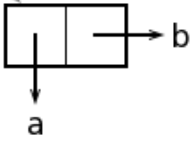
\includegraphics[width=0.25\textwidth]{img/img3.png}
		\caption{Результат cons.} }
\end{figure}

list - не имеет фиксированное количество аргументов. 
Создает список, у которого голова - это первый аргумент,
хвост - все остальные аргументы.
\begin{lstlisting}[language=Lisp]
(list 'a 'b) 				;; (A B)
(list 'a 'b 'v '(c d) 'd) 	;; (A B V (C D) D)
\end{lstlisting}

\begin{figure}[ht!]
	\centering{
		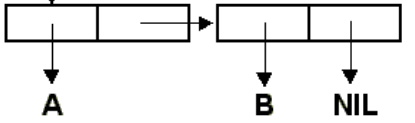
\includegraphics[width=0.5\textwidth]{img/img2.png}
		\caption{Результат list.} }
\end{figure}

\textbf{cons} - имеет фиксированное число аргументов и более экономный по памяти.

\textbf{Ядро} - основные действия, которые наиболее часто используются. Ядро шире, чем базис.